\chapter{3D Foot Placement Estimator and Gait Generation} % (fold)
\label{cha:simulations}

This chapter extends the Foot Placement Estimator (FPE) algorithm for 3D bipedal robots. Section~\ref{sec:extension_to_3d} presents the method of extending the existing 2D theory (reviewed in Section~\ref{sub:related_foot_placement}) to 3D movement. The proposed algorithm selects a 2D plane in the chosen direction of motion and generates trajectories to produce a forward momentum along the plane. A whole body motion control framework coupled with a finite state machine is used to track the generated trajectories and form complete gait cycles. The toolchain described in the preivous chapter is used to generate dynamic simulations for the 14 DOF bipedal robot and the proposed extension to 3D is validated (Section~\ref{sec:simulations_and_results}).

\section{FPE Extension to 3D} % (fold)
\label{sec:extension_to_3d}

In order to extend the FPE approach to the 3D case, the concept of generating complete gait cycles described in Section~\ref{sub:gait_cycles} is revisted. The primary goal of the first three states in each step cycle (\textbf{PUSH}, \textbf{LIFT} and \textbf{SWING}) is to force the biped into an unstable configuration so that the FPE algorithm can be used to regain stability in the terminal state (\textbf{DROP}).

To extend the 2D algorithm to the general 3D case, we begin by selecting a suitable plane in 3D space as the sagittal plane. The off-sagittal plane is perpendicular to the sagittal plane and the ground.  In the proposed approach, the goal of each step cycle is to control the motion of a 3D bipedal robot to generate a forward moving momentum \emph{along} the selected sagittal plane. Upon entering the terminal state, the FPE equation (\ref{eq:fpe}) is solved on the selected plane to determine the swing foot placement and ultimately regain stability. Unlike the 2D case, consider a 3D bipedal robot with finite foot length and width rather than a biped with point feet as demonstrated in \cite{Wight:2008vt}. The larger size of the region of support increases robustness to these approximation errors. 

The remainder of this thesis assumes a 3D bipedal robot with $n$ actuated degrees of freedom (DOF) and $n+6$ generalized coordinates defined by (\ref{eq:eom1}). 

\subsection{Sagittal Plane} % (fold)
\label{sub:sagittal_plane}
To select an appropriate sagittal plane for a 3D bipedal robot, a vertical plane which lies between the current position of the stance foot and the desired direction of motion is chosen. For a 3D biped walking in a forward motion, this plane is chosen as the the vertical plane passing through the midpoint between the hips and parallel to the direction of forward progress. For side-stepping motion, the coronal plane through the stance foot in the direction of the side step is chosen as the sagittal plane. The selection of the sagittal plane for 3D bipedal robots is illustrated in Figure~\ref{fig:sagittal_plane} for these two situations. 

\begin{figure}[!h]
	\begin{center}
	\subfigure{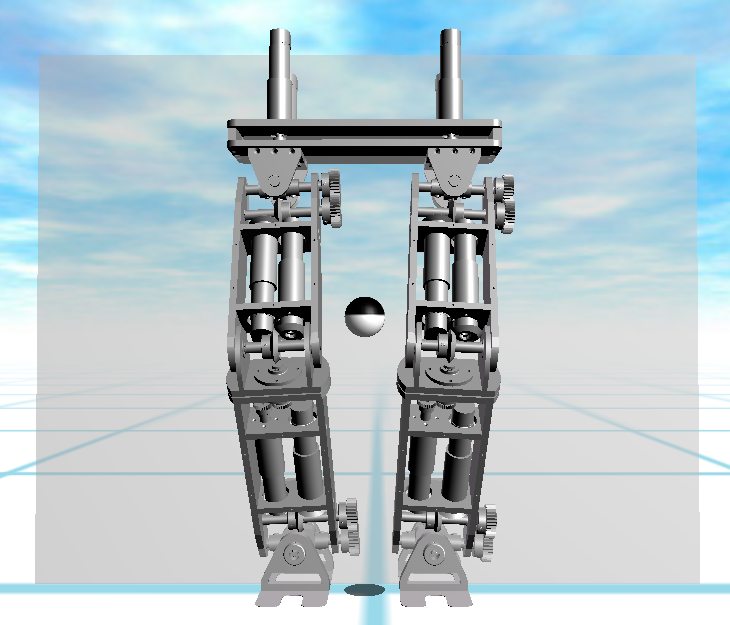
\includegraphics[scale=0.52]{fig/fpe/fpeplanesidestep.png}} 
	\subfigure{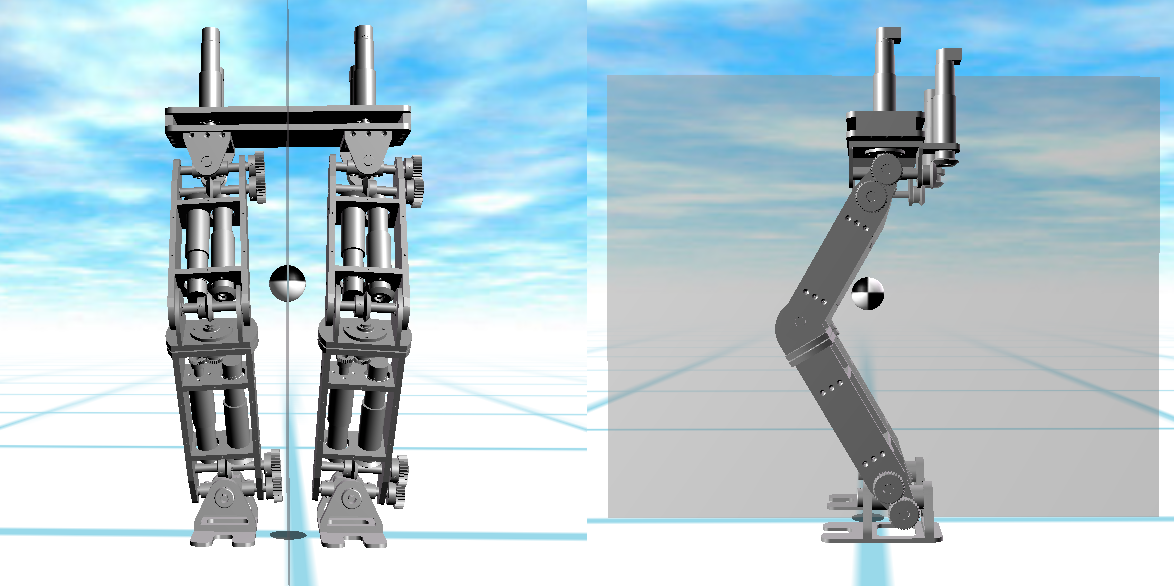
\includegraphics[scale=0.52]{fig/fpe/fpeplaneforwardwalk.png}}
	\end{center}
  	\caption{Sagittal plane selection shown as translucent gray for side-stepping (left) and forward walking (right).}
	\label{fig:sagittal_plane}
\end{figure}

The motion of the biped is controlled based on the selected plane for the duration of the step cycle. During gait initiation, the lines from the COM to the contact points are of length $L$, and the leg separation angle is $\beta$ (similar to the planar case). If the motion of the biped is constrained along this plane, the FPE angle $\phi$ can be used to determine foot placement to regain stability. The parameters required to solve the FPE equation are projected onto the selected plane (additional details are provided in Section~\ref{sub:computing_fpe_parameters}).

Upon impact, the angle $\phi$ converges to $\beta/2$ and a new sagittal plane can be selected for the subsequent step cycle prior to the swing leg entering the \textbf{PUSH} state. Once selected, the stance foot is rotated for alignment and swing leg trajectories can be generated along the plane. By selecting a plane between the current and desired directions of motion, this approach can achieve turning with each step.

% subsection sagittal_plane (end)

\subsection{Trajectory Generation} % (fold)
\label{sub:trajectory_generation}
Once the sagittal plane has been identified at the beginning of each step cycle, appropriate task space trajectories must be generated for the COM ($x_{COM}$) and the swing foot ($x_{SWING}$). In the 2D case, the main goal of the initial states \textbf{PUSH}, \textbf{LIFT} and \textbf{SWING} was to achieve enough forward motion to destabilize the biped. In the 3D case, the robot must also remain stable in the off-sagittal plane while achieving the desired sagittal plane motion. If the ZMP leaves the region of support formed by the stance foot as the swing foot is lifted, the biped begins to fall in the off-sagittal plane and the solution to the 2D FPE equation is insufficient to maintain stable gait. To ensure both forward progress and off-sagittal plane stability, the generated trajectories for $x_{COM}$ are shown in Figure~\ref{fig:comtraj3d}. \\

\begin{figure}[!h]
	\centering
    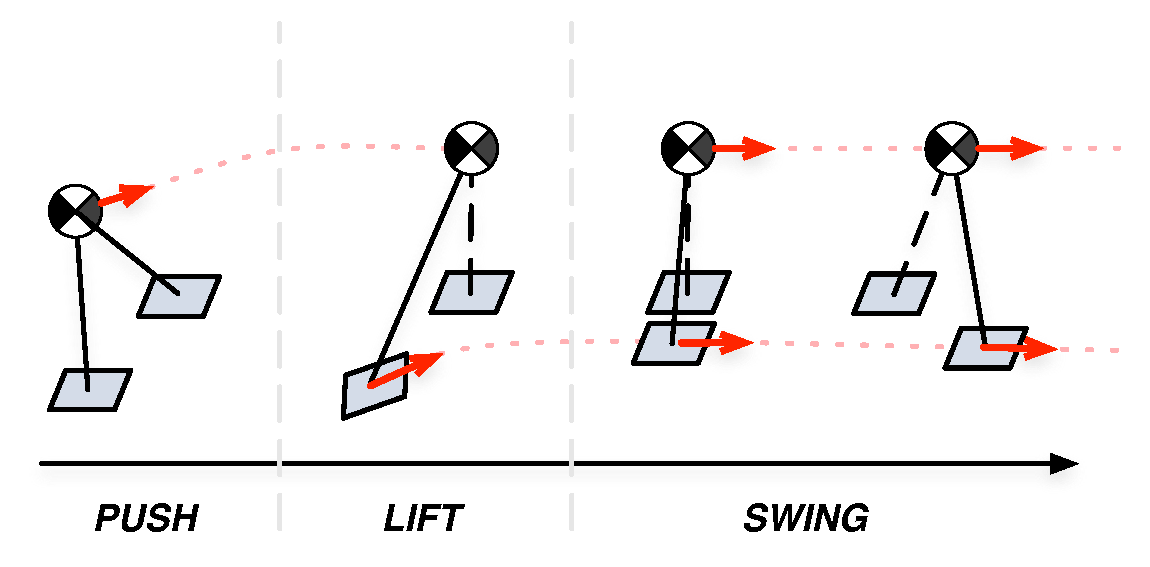
\includegraphics[scale=0.8]{fig/fpe/comtraj3d.eps} 
  	\caption{Trajectory for $x_{COM}$ to ensure forward progress and off-sagittal stability for 3D FPE.}
	\label{fig:comtraj3d}
\end{figure}

\textbf{PUSH}: $x_{COM}$ is moved above the leading stance foot to maintain stability in the off-sagittal and sagittal planes.

\textbf{LIFT}: $x_{COM}$ is held at its current location (above stance foot) while the swing foot is lifted from the ground to achieve sufficient clearance.

\textbf{SWING}: $x_{COM}$ is held in place until the swing foot is aligned with the stance foot in the off-sagittal plane. At this point the $x_{COM}$ is deliberately pushed outside the region of support in the sagittal plane direction. \\

A similar approach is used to generate trajectories for $x_{SWING}$ to achieve the desired behaviour of generating enough momentum to destabilize the biped in the sagittal plane while maintaining stability in the off-sagittal plane. Trajectories for $x_{SWING}$ (illustrated in Figure~\ref{fig:swingfoottraj}) are always computed to align with the sagittal plane formed by the stance foot at the start of the step cycle. This ensures that the solution to the 2D FPE equation remains valid as the \textbf{DROP} state is entered. \\

\textbf{PUSH}: $x_{SWING}$ is held in place as the $x_{COM}$ trajectory is tracked.

\textbf{LIFT}: $x_{SWING}$ follows a ramped trajectory to simultaneously raise the foot off the ground and move it forward in the sagittal plane.

\textbf{SWING}: $x_{SWING}$ follows a straight line trajectory at a specific ground clearance (shown as $h_{LIFT}$ on Figure~\ref{fig:swingfoottraj}) until it reaches the FPE angle $\phi$ or the biped is unstable. \\

\begin{figure}[!h]
	\centering
    \includegraphics[scale=0.8]{fig/fpe/swingfoottraj.eps} 
  	\caption{Trajectory for $x_{SWING}$ along the selected (sagittal) $xz$-plane for 3D FPE.}
	\label{fig:swingfoottraj}
\end{figure}

The ramp trajectory used to raise the swing foot during \textbf{LIFT} should be parameterized in terms of the velocity of the FPE point so that this state transitions faster in the event of larger disturbances (since the biped would have a shorter amount of time to swing the foot over and catch itself).

Depending on the supervisory control mode (i.e. \textbf{WALK} or \textbf{STAND}), the swing leg trajectory can be adjusted to implicitly achieve a desired goal. During \textbf{WALK} mode, the swing foot trajectory tracks a point on the ground slightly behind the FPE point. This under stepping behaviour results in the biped having enough forward moving momentum when the swing foot comes in contact with the ground such that the biped is unstable. As a result, the FPE point is continuously moving forward causing the state machine to transition into the opposing foot's \textbf{LIFT} state upon contact. In the \textbf{STAND} mode, the swing foot trajectory is adjusted to overstep the FPE point so that the biped comes to a stop following this step.

% subsection task_space_trajectory_generation (end)

\subsection{Control Strategy} % (fold)
\label{sub:control_strategy}

A hybrid control strategy is used to simultaneously maintain stability in the off-sagittal plane, achieve sufficient forward momentum along a selected sagittal plane and ultimately track the FPE location to regain stability by taking a step. Similar to the approach presented in \cite{Wight:2008vt}, this approach uses a state machine to transition through the step sequence with each state having a local controller.

During the initial states of the step cycle, whole body motion control is used to track the $x_{COM}$ and $x_{SWING}$ trajectories described in  Section~\ref{sub:trajectory_generation}. To generate the corresponding joint level trajectories, the Jacobian matrix is used to map between the task space and the joint space velocities:

\begin{IEEEeqnarray}{rCl}
	\label{eq:jmap}
	J & = & \begin{bmatrix} \partial q_{act} & \partial x_{base} \\ \end{bmatrix}_{m \times (n+6)}
\end{IEEEeqnarray}

A prioritized task space control scheme is used to generate joint level trajectories which simultaneously achieve state goals while satisfying the highest priority constraint (i.e. holding the $x_{COM}$ position). The state-dependent joint level trajectories can be computed by projecting the lower priority task space goals onto the null space of higher priorities:

\begin{eqnarray}
	\label{eq:priori}
	\dot{q}_{ref} = S(J_{H}^{\#} \dot{x}_{H} + N_{H} J_{L}^{\#} \dot{x}_{L})
\end{eqnarray}

Where, $S = \begin{bmatrix} I_{n \times n} & 0_{n \times 6} \\ \end{bmatrix}$ is the actuator selection matrix for (\ref{eq:gentau}), $J^{\#}$ is the psuedoinverse of the Jacobian $J$, $\dot{q}_{ref}$ is the reference joint velocity, and $\dot{x}_H$ and $dot{x}_L$ are the high and low priority task space velocities, respectively. $J_{H}$ are $J_{L}$ are the corresponding high and low priority Jacobians, and $N_{H} = I - J_{H}^{\#} J_{H}$ is the null space projection matrix. The reference joint velocities are integrated to obtain the reference command signal to be tracked by high gain local Proportional-Derivative (PD) controllers. The specific prioritization of each state is discussed in Section~\ref{sub:joint_level_control}.

When the biped enters the terminal state, the hybrid control strategy switches to directly computing the joint level commands using inverse kinematics. The PD controller gains of the stance foot ankle are set to $K_{P} = K_{D} = 0$ to allow the biped to pivot and fall forward. Simultaneously, the inverse kinematics for the swing leg is solved directly to track the FPE point along the selected sagittal plane.
% subsection control_strategy (end)

\subsection{State Dependent Controllers} % (fold)
\label{sub:joint_level_control}
This section presents the specific controller formulation used during each state of the gait cycle.

\subsubsection{\textbf{STAND}} % (fold)
\label{ssub:stand}
The goal during this state is to maintain the COM position at the geometric centroid of both feet. In order to remain stable under small disturbances, the Jacobian under double support phase is used to compensate for the error $\Delta x_{COM}$ in the X and Y directions.

\begin{IEEEeqnarray}{rClrCl}
	J_{H} & = &
	\begin{bmatrix}
		J_{Stand} \\
		J_{Swing} \\
		J_{COM} \\
	\end{bmatrix}  &
	\dot{x}_{H} & = &
	\begin{bmatrix}
		0 \\
		0 \\
		\dot{x}_{COM} \\
	\end{bmatrix} \nonumber \\
	J_{L} & = &
	\begin{bmatrix}
		0 \\
	\end{bmatrix}  &
	\dot{x}_{L} & = &
	\begin{bmatrix}
		0 \\
	\end{bmatrix} \nonumber \\
\end{IEEEeqnarray}

% subsubsection stand (end)

\subsubsection{\textbf{PUSH}} % (fold)
\label{ssub:push}
The goal during this state is to track the trajectory generated for $x_{COM}$ to move to the stance foot support region while remaining in the double support phase. An augmented Jacobian matrix is used to track the trajectory while simultaneously maintaining the foothold constraints.

\begin{IEEEeqnarray}{rClrCl}
	J_{H} & = &
	\begin{bmatrix}
		J_{Stand} \\
		J_{Swing} \\
		J_{COM} \\
	\end{bmatrix}  &
	\dot{x}_{H} & = &
	\begin{bmatrix}
		0 \\
		0 \\
		\dot{x}_{COM} \\
	\end{bmatrix} \nonumber \\
	J_{L} & = &
	\begin{bmatrix}
		0 \\
	\end{bmatrix}  &
	\dot{x}_{L} & = &
	\begin{bmatrix}
		0 \\
	\end{bmatrix} \nonumber \\
\end{IEEEeqnarray}

The joint level reference velocities are calculated from (\ref{eq:priori}) and integrated to obtain the position command.

% subsubsection push (end)

\subsubsection{\textbf{LIFT}} % (fold)
\label{ssub:lift}
In the lift stage, the highest priority task is maintaining the foothold of the stance foot, holding the $x_{COM}$ directly above it and simultaneously raising the swing foot from the ground. The key challenge in this state is that lifting the swing foot can potentially cause the centre of pressure to leave the support region formed by the contact points of the stance foot. The prioritized task space control scheme is used to generate joint level commands to track the $x_{SWING}$ trajectory while satisfying the higher priority goal of maintaining the foothold and balance.

\begin{IEEEeqnarray}{rClrCl}
	J_{H} & = &
	\begin{bmatrix}
		J_{Stance} \\
		J_{COM} \\
	\end{bmatrix} &
	\dot{x}_{H} & = &
	\begin{bmatrix}
		0 \\
		\dot{x}_{COM} \\
	\end{bmatrix} \nonumber \\
	J_{L} & = &
	\begin{bmatrix}
		J_{Swing} \\
	\end{bmatrix}  &
	\dot{x}_{L} & = &
	\begin{bmatrix}
		\dot{x}_{Swing} \\
	\end{bmatrix} \nonumber \\
\end{IEEEeqnarray}

The joint level reference velocities are calculated from (\ref{eq:priori}) and integrated to obtain the position command.

% subsubsection lift (end)

\subsubsection{\textbf{SWING}} % (fold)
\label{ssub:swing}


At this point, the goal of the control approach is to generate a forward moving momentum along the selected sagittal plane. This deliberately destabilizes the biped by pushing $x_{COM}$ outside the region of support in the chosen direction of motion. The task space prioritization in this state remains consistent with the previous state until the biped is unstable, at which point the control strategy enters the terminal \textbf{DROP} state.

\begin{IEEEeqnarray}{rClrCl}
	J_{H} & = &
	\begin{bmatrix}
		J_{Stance} \\
		J_{Swing} \\
	\end{bmatrix} &
	\dot{x}_{H} & = &
	\begin{bmatrix}
		0 \\
		\dot{x}_{Swing} \\
	\end{bmatrix} \nonumber \\
	J_{L} & = &
	\begin{bmatrix}
		J_{COM} \\
	\end{bmatrix}  &
	\dot{x}_{L} & = &
	\begin{bmatrix}
		\dot{x}_{COM} \\
	\end{bmatrix} \nonumber \\
\end{IEEEeqnarray}

The joint level reference velocities are calculated from (\ref{eq:priori}) and integrated to obtain the position command.
% subsubsection swing (end)

\subsubsection{\textbf{DROP}} % (fold)
\label{ssub:drop}
In this terminal state, the Jacobian is used to track the fixed stance foot position and the generated swing foot trajectory to track the FPE point on the ground. Since the ZMP is outside of the region of foot support during this state, the torso is treated as a fixed base link and compute the Jacobian matrix of each foot.

\begin{IEEEeqnarray}{rClrCl}
	J_{H} & = &
	\begin{bmatrix}
		J_{Stance} \\
		J_{Swing} \\
	\end{bmatrix} &
	\dot{x}_{H} & = &
	\begin{bmatrix}
		\dot{x}_{Stand} \\
		\dot{x}_{Swing} \\
	\end{bmatrix} \nonumber \\
	J_{L} & = &
	\begin{bmatrix}
		0 \\
	\end{bmatrix}  &
	\dot{x}_{L} & = &
	\begin{bmatrix}
		0 \\
	\end{bmatrix} \nonumber \\
\end{IEEEeqnarray}

\subsubsection{\textbf{CONTACT STABILIZATION}} 

With an arbitrary 3D biped with finite sized feet, it is possible for the biped to land on the edge of the foot instead of landing perfectly above the FPE point on the ground. Once ground contact is made, the solution to the FPE equation is no longer valid (since a real biped will not have instantaneous transfer of balance). To handle this behaviour, a stabilization substate is used where the joint level control is computed directly. At this point, trajectories are generated for the ankles to align the surface of the foot with the ground and switch to high gain PD control for tracking. This ensures that both feet are in full contact with the ground prior to executing the opposite leg's gait sequence. The biped-ground contact interface is shown before and after the stabilization substate in Figure~\ref{fig:contact_stabilization}. 

\begin{figure}[!h]
	\begin{center}
	\subfigure{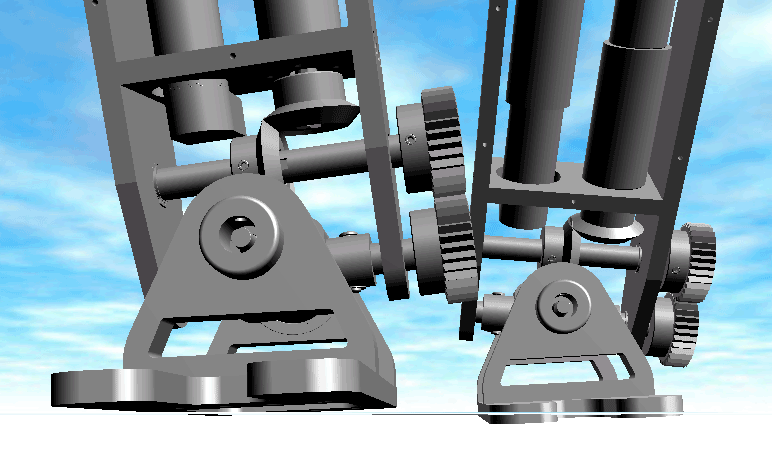
\includegraphics[scale=0.29]{fig/fpe/prestabilization.png}} 
	\subfigure{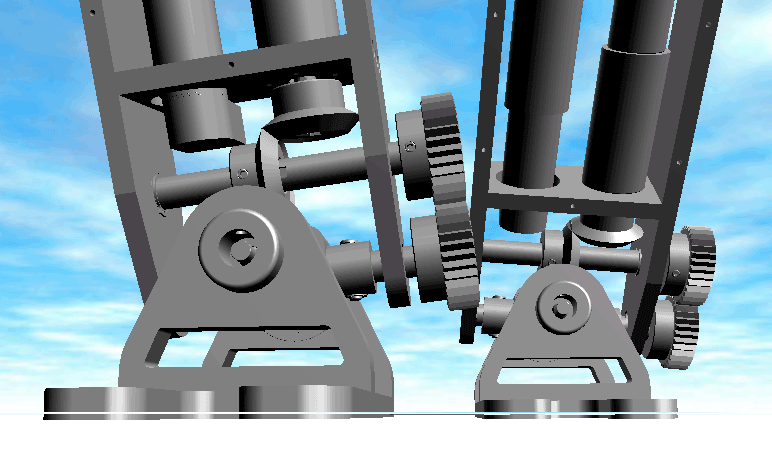
\includegraphics[scale=0.29]{fig/fpe/poststabilization.png}}
	\end{center}
  	\caption{Ground-foot contact shown for before (left) and after (right) contact stabilization.}
	\label{fig:contact_stabilization}
\end{figure}


% subsubsection drop (end)

% subsection joint_level_control (end)

\subsection{Computing the FPE Parameters} % (fold)
\label{sub:computing_fpe_parameters}
The 2D FPE equation (\ref{eq:fpe}) requires the total inertia about the COM ($I_{COM}$) and average angular velocity about the pivoted fixed foot ($\dot{\theta}_{avg}$). In the 2D case, the moment of inertia for link $k$ is a scalar value since there is only one plane of rotation. The total inertia about the COM is computed by summing the moment of inertia for each link in the system. In the 3D case, the moment of inertia for each link is a $3\times3$ tensor: 

\begin{equation}
	\begin{aligned}
		{I_k} = \left[ {\begin{array}{*{20}{c}}
{{I_{xx}}}&{{I_{xy}}}&{{I_{xz}}}\\
{{I_{yx}}}&{{I_{yy}}}&{{I_{yz}}}\\
{{I_{zx}}}&{{I_{zy}}}&{{I_{zz}}}
\end{array}} \right]
	\end{aligned}
\end{equation}

The inertia tensor of each link is taken at the COM aligned with the local coordinate system. If the $xz$-plane is selected as the sagittal plane in 3D space, the moment of inertia of link $k$ is the $I_{yy}$ term. However, in the 3D case the motion of the biped is no longer fixed to a single plane of rotation. By attaching a fixed coordinate frame to the selected sagittal plane at the start of each step, the orientation of the sagittal plane can be expressed as a $3\times3$ rotation matrix $R$. The local inertia tensor can be rotated into the selected sagittal plane's coordinate frame by: 

\begin{equation}
	\begin{aligned}
		{I_{k,sagittal}} = R \cdot {I_k} \cdot {R^T}
	\end{aligned}
	\label{eq:isagittal}
\end{equation}

Then the effective moment of inertia of each link \emph{projected on to the selected sagittal plane} can be obtained by transforming the inertia tensor with (\ref{eq:isagittal}) and pulling out the $I_{yy}$ term, $I_{k,yy}$. The total inertia about the COM can then be computed by summing the effective inertia of each link on the sagittal plane: 

\begin{equation}
	\begin{aligned}
		{I_{COM}} = \sum\limits_{k = 1}^n {{I_{k,yy}}}
	\end{aligned}
	\label{eq:icom_3d}
\end{equation}

The average angular velocity is computed as a weighted sum of the inertia of each link \cite{Wight:2008ii}. In the 3D case, the same equation is used with the \emph{effective} moment of inertia of each link on the sagittal plane: 

\begin{equation}
	\begin{aligned}
		{\dot \theta _{avg}} = \frac{{\sum\limits_{k = 1}^n {{I_{k,yy}}} {{\dot \theta }_k}}}{{\sum\limits_{k = 1}^n {{I_{k,yy}}} }}
	\end{aligned}
	\label{eq:wavg_3d}
\end{equation}

The angular velocity of each link ${\dot{\theta}_k}$ is obtained by rotating the joint velocity (expressed as a $3\times1$ vector with $\dot{q}_k$ in the row represented by its local axis of rotation) to the fixed frame of the sagittal plane. 

The parameters computed with (\ref{eq:icom_3d}) and (\ref{eq:wavg_3d}) are plugged in to the 2D FPE equation (\ref{eq:fpe}) and the solution ($\phi$) is obtained with a non-linear equation solver. 
% subsection computing_fpe_parameters (end)

% section extension_to_3d (end)

\section{Simulations and Results} % (fold)
\label{sec:simulations_and_results}

The proposed control strategy to extend the FPE theory to 3D was implemented in simulation on a 14 DOF lower body bipedal robot. Each state of the control strategy was implemented in the Matlab/Simulink environment with the multibody dynamics simulation by SimMechanics. Accurate kinematic and dynamic properties of the physical robot were taken directly from the CAD model through the toolchain model generation process (as discussed in Section~\ref{sec:model_generation}). The controller diagram shown in Figure~\ref{fig:fpecontroller} implements the control strategy presented in this section. The subsystems from the outer most loop working inwards are described as follows: 

\begin{figure*}[!b]
	%\centering
    \centerline{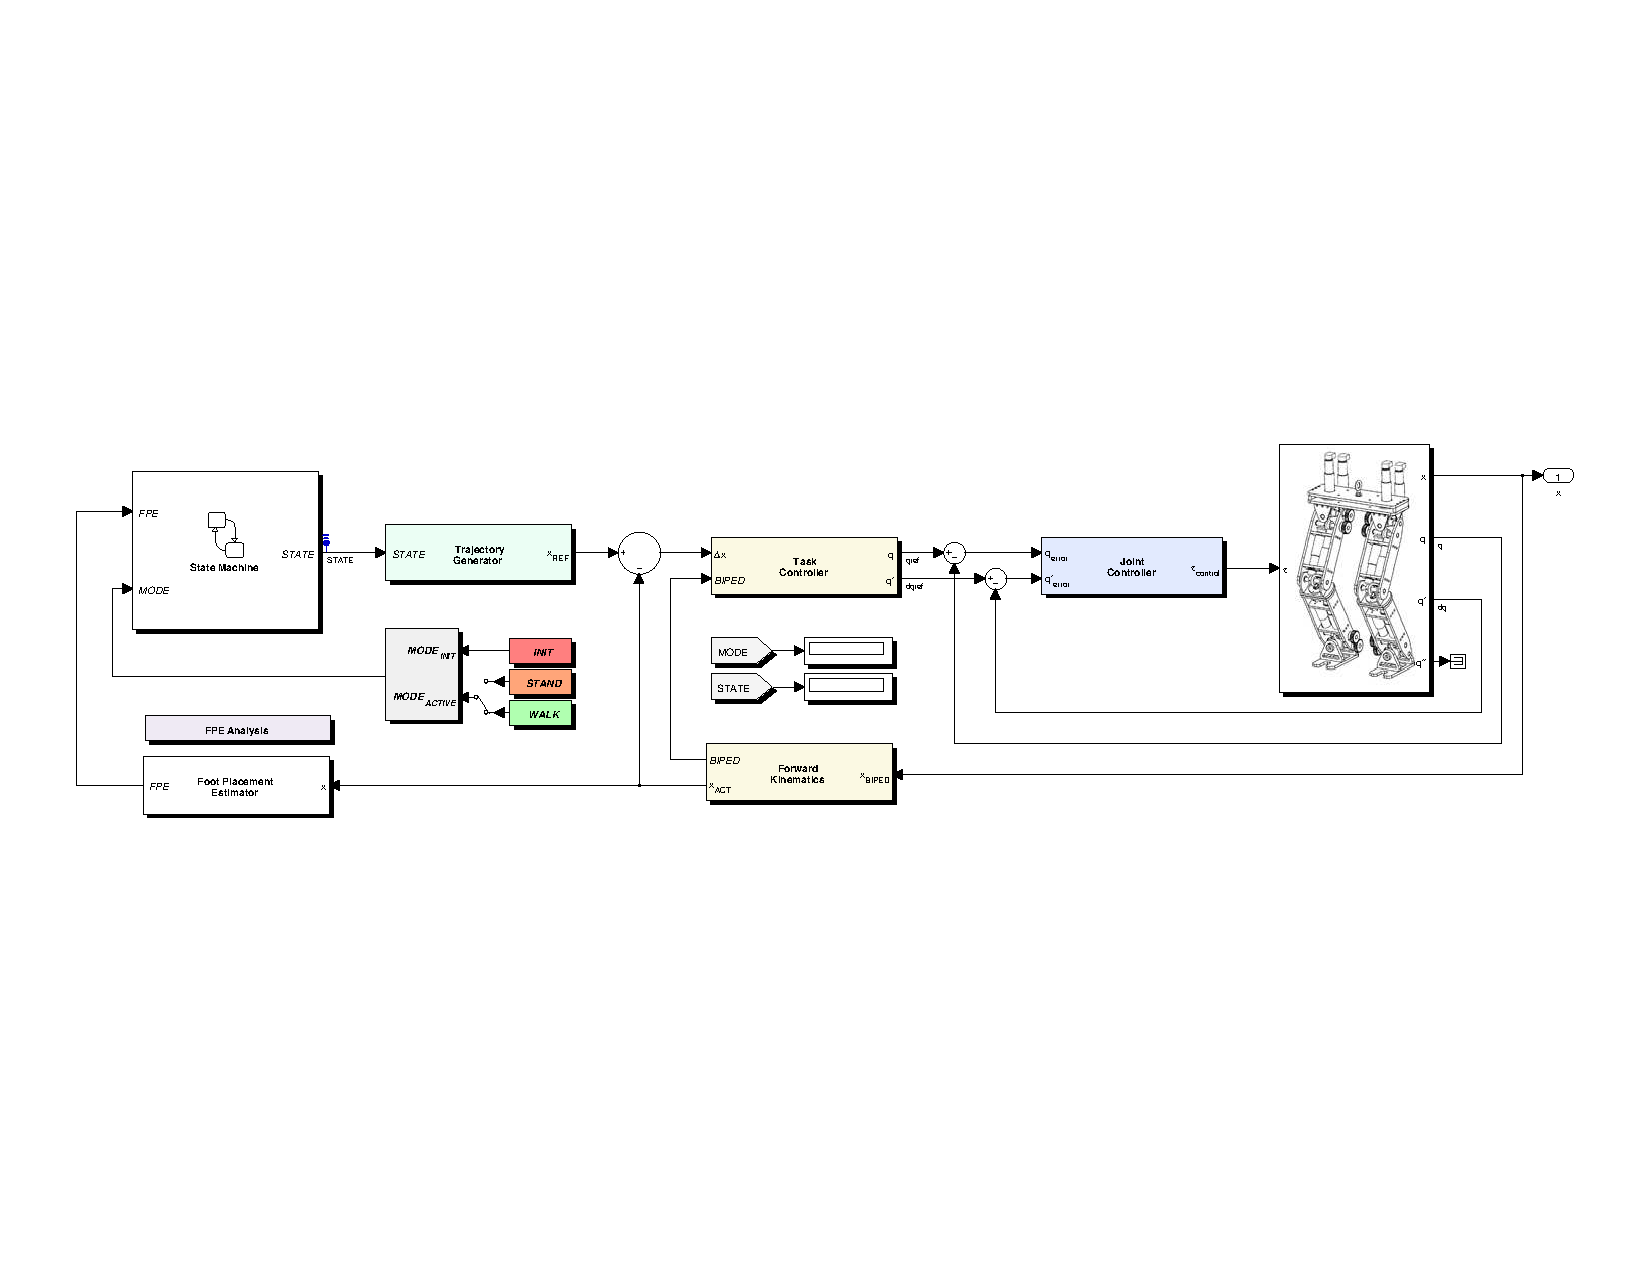
\includegraphics[trim = 12mm 75mm 12mm 75mm,clip,width=18cm]{fig/simulations/fpecontroller.pdf}}
  	\caption{Controller diagram of 3D FPE based walking control strategy implemented in Simulink.}
	\label{fig:fpecontroller}
\end{figure*}

\begin{enumerate}
	\item \textbf{State Machine} \\ 
	Finite state machine logic was implemented in Stateflow as shown in Figure~\ref{fig:stateflow}. The state names follow the same convention as the 2D FPE case (shown in Figure~\ref{fig:statemachine}) while the transition logic is updated for the 3D case described in Section~\ref{sub:joint_level_control}.  \\

	\item \textbf{Trajectory Generator} \\ 
	Generates the task space COM ($x_{COM}$) and the swing foot ($x_{SWING}$) trajectories detailed in Section~\ref{sub:trajectory_generation} based on the current state of the controller. Also uses the higher level supervisory control mode (i.e. \textbf{WALK} or \textbf{STAND}) to adjust the trajectory generation for understepping/overstepping the FPE point. \\

	\item \textbf{Foot Placement Estimator} \\ 
	Computes the FPE parameters about the COM ($I_{COM}$, $\dot{\theta}_{avg}$) for the 3D case (detailed in Section~\ref{sub:computing_fpe_parameters}) and solves the FPE equation (\ref{eq:fpe}) using a numerical methods-based nonlinear solver from \cite{Wight:2008vt}. \\

	\item \textbf{Task Controller} \\ 
	Provides the state dependent control logic for the whole body motion control framework in Section~\ref{sub:control_strategy}. The resulting joint space velocities are integrated to obtain the joint position reference command. The contact stabilization substate used in the second half of \textbf{DROP} is also implemented here to generate joint level trajectories directly. \\

	\item \textbf{Joint Controller} \\ 
	High gain joint level PD controllers with gain scheduling based on the current state of the control strategy. The output of this block ($\vtau$) is used to drive the forward dynamics simulation generated with the toolchain. \\

\end{enumerate}

\begin{figure}[!h]
	\centering
    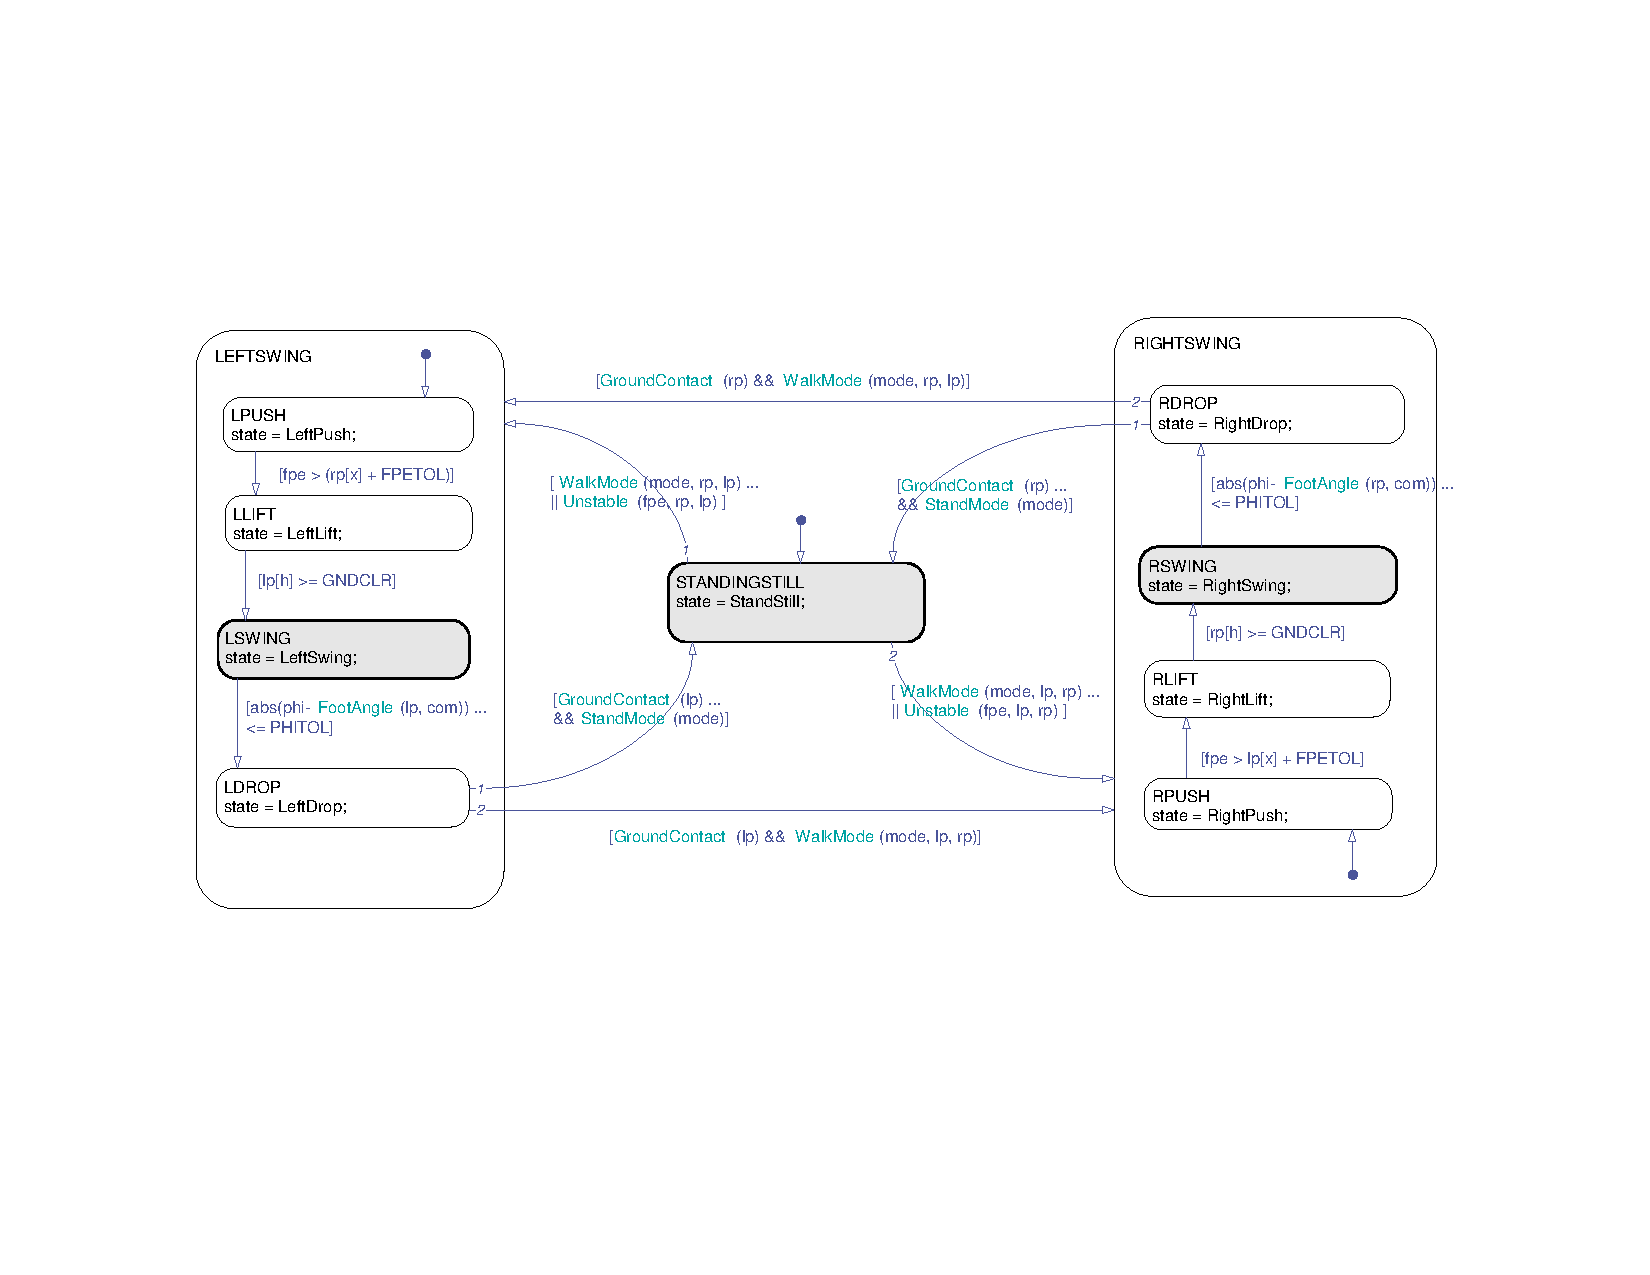
\includegraphics[trim = 30mm 60mm 25mm 53mm,clip,width=17cm]{fig/simulations/statemachine.pdf} 
  	\caption{Finite state machine implemented in Stateflow for 3D FPE-based walking control strategy.}
	\label{fig:stateflow}
\end{figure}

The simulations are executed with a fixed step Runge-Kutta solver at 1KHz. The forward dynamics generated with the toolchain drive the simultaneous 3D visualizations in an external viewer application.  

\subsection{Contact Modeling} % (fold)
\label{sub:full_contact_modeling}
The initial spring-damper contact model discussed in Section~\ref{sub:initial_contact_modeling} was replaced with a more complex version to accurately model the ground/foot dynamics. The Hunt and Crossley contact model \cite{hunt1975coefficient,gilardi2002literature} generates a normal force using a non-linear spring-damper system defined by: 

\begin{equation}
	\label{eq:contacthc}
	{F_{normal}} = b{z^p}{\dot z^q} + k{z^n}
\end{equation}

Where $z$, $\dot{z}$ are the penetration depth position and velocity, respectively. The constants $k$, $b$ are the spring-damper coefficients and $n$, $p$, $q$ are tunable constants. Equation (\ref{eq:contacthc}) provides the ground reaction force in the normal direction only. The tangential (frictional) contact forces were modeled by: 


\begin{equation}
	\label{eq:contactfr}
	{F_{tangential}} = f{\dot x}
\end{equation}

Where $\dot x$ is the tangential velocity of the contact point (in the $x$ and $y$ directions) and $f$ is a tunable constant. The forces generated by (\ref{eq:contacthc}) and (\ref{eq:contactfr}) ensure that there are no discontinuities when ground contact is made. A seperate dynamic simulation model was generated to tune the contact model constants to emulate a stiff ground. The final (tuned) parameters used for dynamic simulations are provided in Table~\ref{tab:contactk}.

\begin{table}[!h]
  \centering
  \caption{Tuned contact model constants.}
    \begin{tabular}{cc}
    \addlinespace
    \toprule
    \textbf{Parameter} & \textbf{Value}\\
    \midrule
	$f$	&	10 \\
    $k$	&	2000 \\
    $b$	&	10 \\
    $p$	&	1.10 \\
    $q$  &	1.00 \\
    $n$	&	2.31 \\
    \bottomrule
    \end{tabular}
  \label{tab:contactk}
\end{table}

It was found that stiffening the ground contact by raising the model constants would produce singularities with fixed time step simulations at 1 KHz. Reducing the time step helped avoid singularities but the simulation runtime drastically increased. 
% subsection contact_modeling (end)

\subsection{Side-to-Side Stepping} % (fold)
\label{sub:3d_simulations}

\begin{figure}[!h]
	\centering
    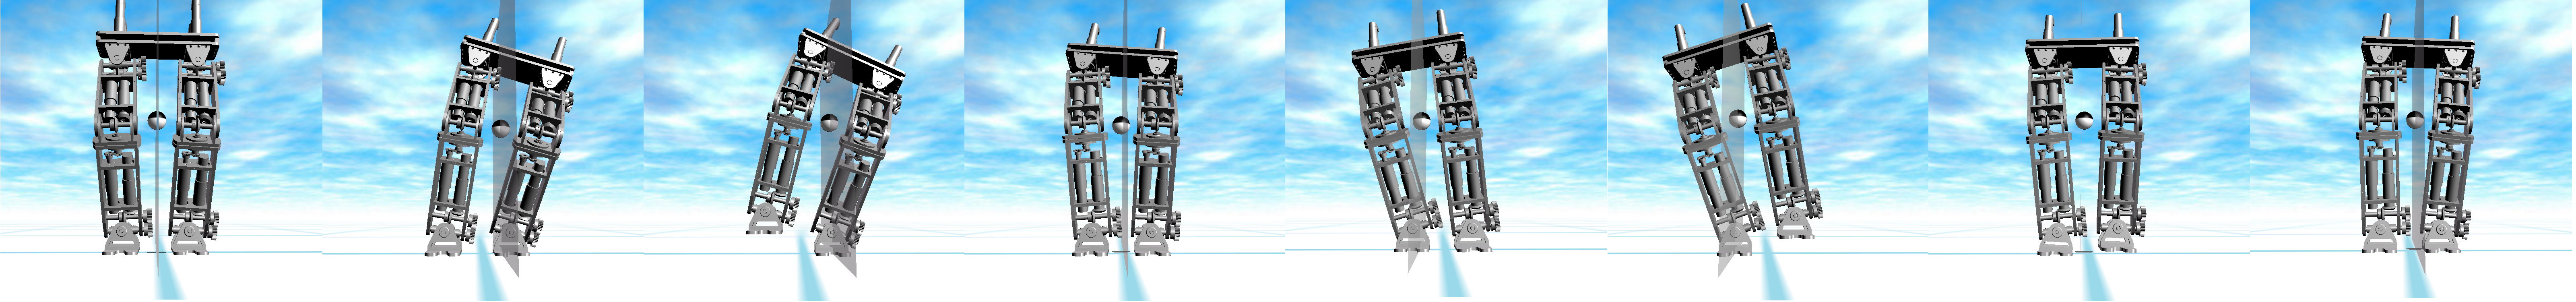
\includegraphics[scale=0.095]{fig/simulations/sidesequence.png}
  	\caption{Frame captures from the realtime 3D visualization while side-to-side stepping.}
	\label{fig:sidesequence}
\end{figure}

To demonstrate the dynamic stability of a 3D biped under this approach, the frontal plane was selected as the sagittal plane. Forward motion along this sagittal plane results in a side-to-side stepping sequence for the biped (as shown in Figure \ref{fig:sidesequence}). The gray plane in the frame captures moves along the Y-direction (biped's frontal plane). The intersection of the gray plane and the ground indicates the FPE point tracked during \textbf{DROP}. 

\begin{figure}[!h]
	\centering
    \includegraphics[scale=0.7]{fig/simulations/sidecomtraj.eps}
  	\caption{COM trajectory being tracked during the complete gait sequence of side stepping.}
	\label{fig:sidecomtraj}
\end{figure}

The resulting $x_{COM}$ trajectories from simulating the side-to-side stepping motion (shown in Figure \ref{fig:sidecomtraj}) demonstrate the stability of the biped through a complete gait sequence. The prioritized motion control framework handles the dynamic switching of constraints (from double support to single support) while generating the appropriate joint level commands for swinging the COM over. The colour coded dotted lines on Figure \ref{fig:sidecomtraj} indicate the boundaries of each foot on the ground. Note that during the \textbf{SWING} state, the COM is pushed outside the region of support (around 11s). This in turn initiates the \textbf{DROP} state where the FPE point is tracked to regain stability.

\begin{figure}[!h]
	\centering
    \includegraphics[scale=0.7]{fig/simulations/sidefpetrack.eps}
  	\caption{Swing foot tracks the a point on the ground given by $FPE + FPE_{offset}$ to ensure overstepping.}
	\label{fig:sidefpetrack}
\end{figure}


In the terminal \textbf{DROP} state, the swing foot trajectory tracks the FPE point on the ground (shown in Figure \ref{fig:sidefpetrack}) with an added offset to ensure that the biped oversteps to guarantee stability (as per the 2D FPE theory). Once ground contact is made (around 11.6s), the stabilization substate is entered and the swing foot trajectory is controlled directly to align the foot with the ground. This causes the biped to rock back and forth (similar to the 2D case) until stability is reached.

\begin{figure}[!h]
	\centering
    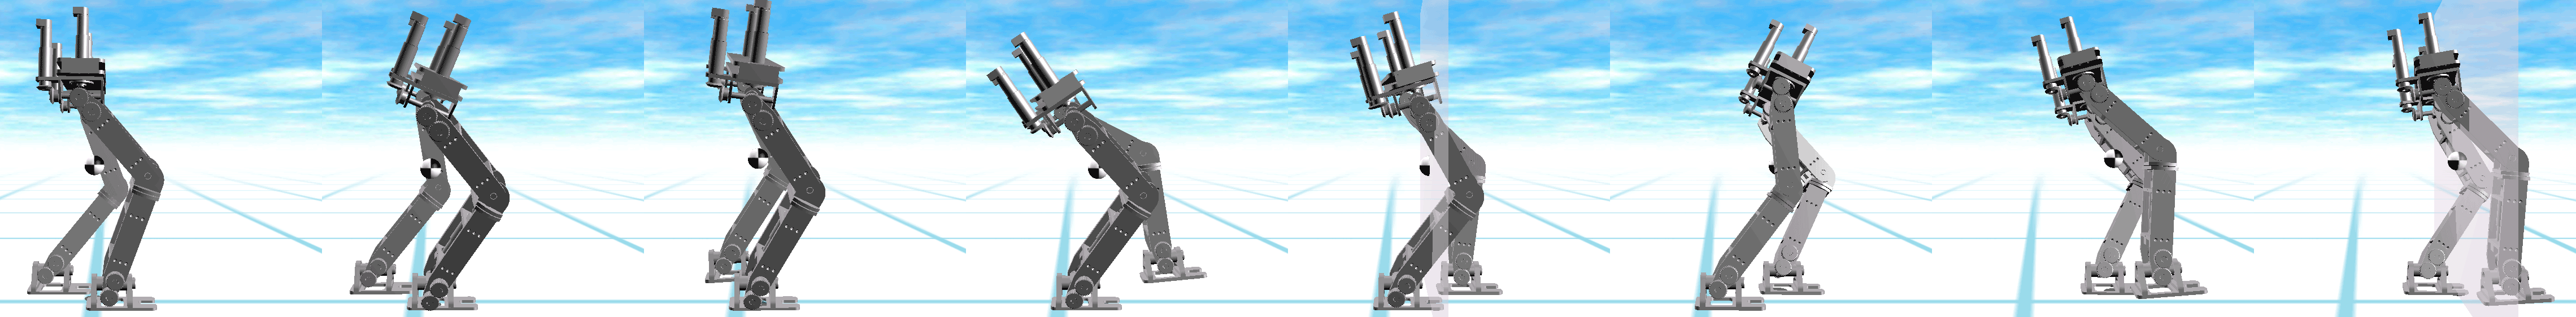
\includegraphics[scale=0.1]{fig/simulations/fwdsequenceside.png}
  	\caption{Frame captures from the realtime 3D visualization with forward walking gait.}
	\label{fig:fwdsequenceside}
\end{figure}

\subsection{Forward Walking Gait} % (fold)
\label{sub:forward_walking_gait}

\begin{figure}[!b]
	\centering
    \includegraphics[scale=0.7]{fig/simulations/fwdcomtraj.eps}
  	\caption{COM and foot trajectories in the direction of forward progress and off-sagittal plane during a complete gait cycle.}
	\label{fig:fwdcomtraj}
\end{figure}

Forward walking is achieved by selecting the biped's sagittal plane as the direction of motion. The frame captures from forward walking simulations are shown in Figure~\ref{fig:fwdsequenceside}. The key challenge is maintaining stability in the off-sagittal plane while the swing foot is raised off the ground during the \textbf{LIFT} state. The $x_{COM}$ trajectories shown in Figure~\ref{fig:fwdcomtraj} demonstrate the dynamic stability in the off-sagittal plane while forward progress is made along the chosen direction of motion. The proposed trajectory generation for $x_{COM}$ illustrated by Figure~\ref{fig:comtraj3d} can be seen at 8s and 22s when the COM is pushed outside the region of support once the swing foot is aligned. 

The alternating foot trajectories on the selected sagittal plane during a complete gait cycle are shown in Figure~\ref{fig:fwdfoottraj}. The first step is taken with the left foot tracking $x_{SWING}$ (between 5-12s). The \textbf{DROP} state is entered around 12s and the left foot tracks a $x_{SWING}$ trajectory given by $FPE + FPE_{offset}$ to ensure over stepping. Once ground contact is made, the contact stabilization state is used to straighten both feet and spread the ground reaction force evenly (around 12-14s). The step cycle begins for the right leg from 15s to complete the gait sequence. 

\begin{figure}[!h]
	\begin{center}
	\subfigure{\includegraphics[scale=0.45]{fig/simulations/fwdlfoottraj.eps}}
	\subfigure{\includegraphics[scale=0.45]{fig/simulations/fwdrfoottraj.eps}}
	\end{center}
  	\caption{Left and right foot trajectories on the selected sagittal plane during a complete gait cycle.}
	\label{fig:fwdfoottraj}
\end{figure}

The FPE trajectory along the forward walking direction is shown in Figure~\ref{fig:fwdfpetraj}. The FPE location on the ground is tracked (with an offset) to regain stability around 12s by the swinging left foot and again around 25s by the swinging right foot. The FPE location also remains safely between the feet during the double support phase after each step is made (approximately 13-15s). 


\begin{figure}[!h]
	\centering
    \includegraphics[scale=0.7]{fig/simulations/fwdfpetraj.eps}
  	\caption{FPE and foot trajectories in the direction of forward progress during a complete gait cycle.}
	\label{fig:fwdfpetraj}
\end{figure}

% subsection forward_walking_gait (end)

% section simulations_and_results (end)

\section{Summary} % (fold)
\label{sec:simulations_summary}
The FPE theory is extended to the 3D case to form dynamically stable gait cycles by selecting a 2D sagittal plane parallel to the desired direction of motion. The primary goal in the 3D case is to generate a forward momentum along this selected sagittal plane. For the duration of the step cycle, the FPE equation is used to determine the appropriate swing foot placement to restore balance from the momentum generated along the plane. A new sagittal plane is selected with each step to enable turning. 

Trajectories are generated for the swing foot and COM position to simultaneously generate the forward momentum along the plane while remaining stable in the off sagittal plane until the \textbf{DROP} state is reached. Upon entering this terminal state, the 3D biped is falling forward in the desired direction of motion and the swing foot tracks the FPE point to restore balance. 

A whole body motion control framework is used to generate the appropriate joint level trajectories during each state of the proposed control strategy. The framework uses a prioritized control scheme where the low priority constraints of each state are projected into the null space of higher priority tasks. This approach handles the dynamic switching of constraints as the biped moves between the single and double support phases. 

The 14 DOF bipedal robot developed in previous chapters is used to demonstrate the control strategy presented in this chapter. Dynamic simulations with 3D visualization are generated directly from the CAD model using the toolchain. The simulations are used to verify the efficacy of the proposed control strategy for side-stepping and forward walking gait. Despite using a more complex contact model, tuning the parameters to accurately model a stiff ground in reality proved to be challenging. This imperfection in the simulation environment highlights the need to develop physical hardware to validate walking control strategies, as presented in the following chapter.
% section discussion (end)

% chapter simulations (end)